\chapter{Экспериментальная часть}
При помощи программы я моделировал нормальное падение моноэнергетического пучка электронов на подложку с нанесенным на неё слоем резиста. Для моделирования использовались электроны с энергией 20 кэВ, подложка была кремниевая, а резист был выполнен ПММА и имел толщину 500 нм.

\begin{figure}[h]
    \center
    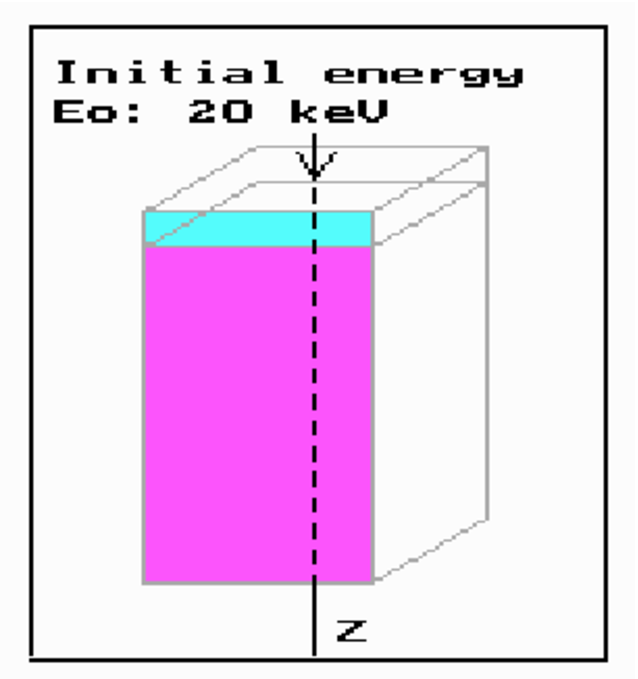
\includegraphics[width=.47\textwidth]{example}
    \caption{Установка для экспериментального рассчета}
    \label{fig:example}
\end{figure}

В налетающем пучке распределение плотноси энергии имеет вид, представленный на рисунке~\ref{fig:beam}.
\begin{figure}[h]
    \center
    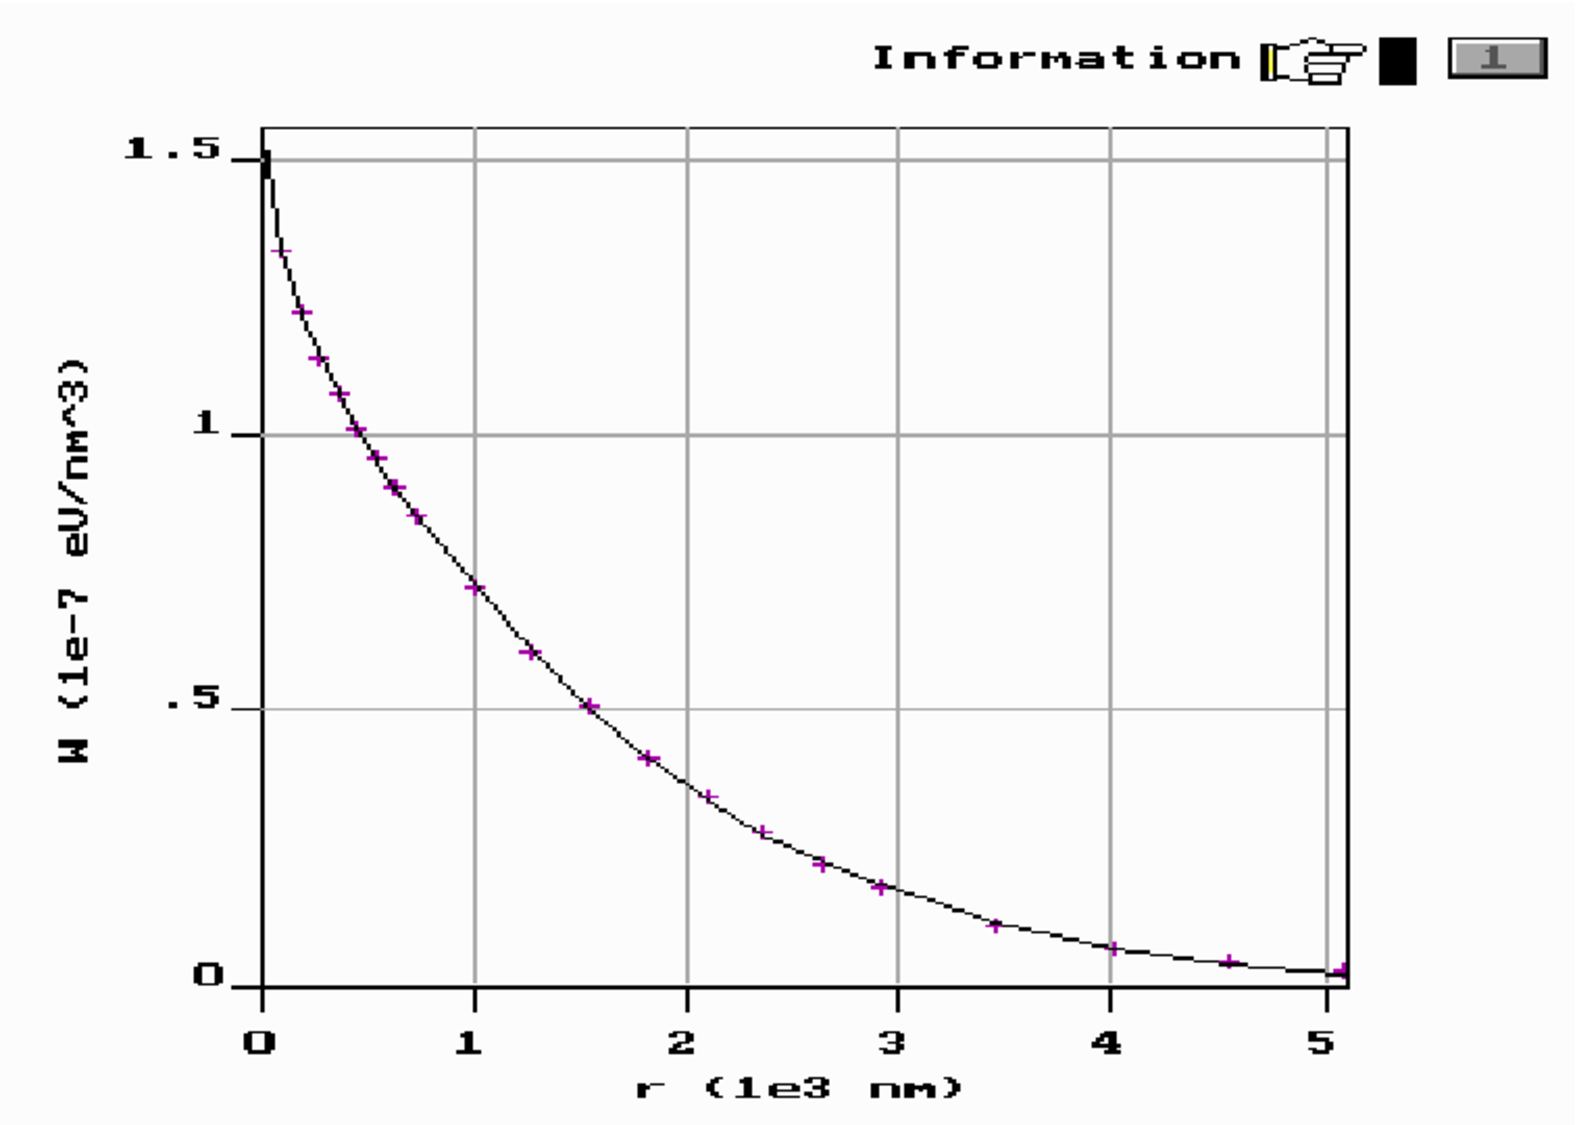
\includegraphics[width=.95\textwidth]{beam}
    \caption{радиальное распределение плотности энергии в налетающем пучке}
    \label{fig:beam}
\end{figure}

Как можно видеть из графика, представленного на рис.~\ref{fig:fluxes}, при данном значении энергии лишь малая часть электронов отражается обратно, в основном они диффундируют.
% здесь можно приплести про эффект близости
\begin{figure}[h]
    \center
    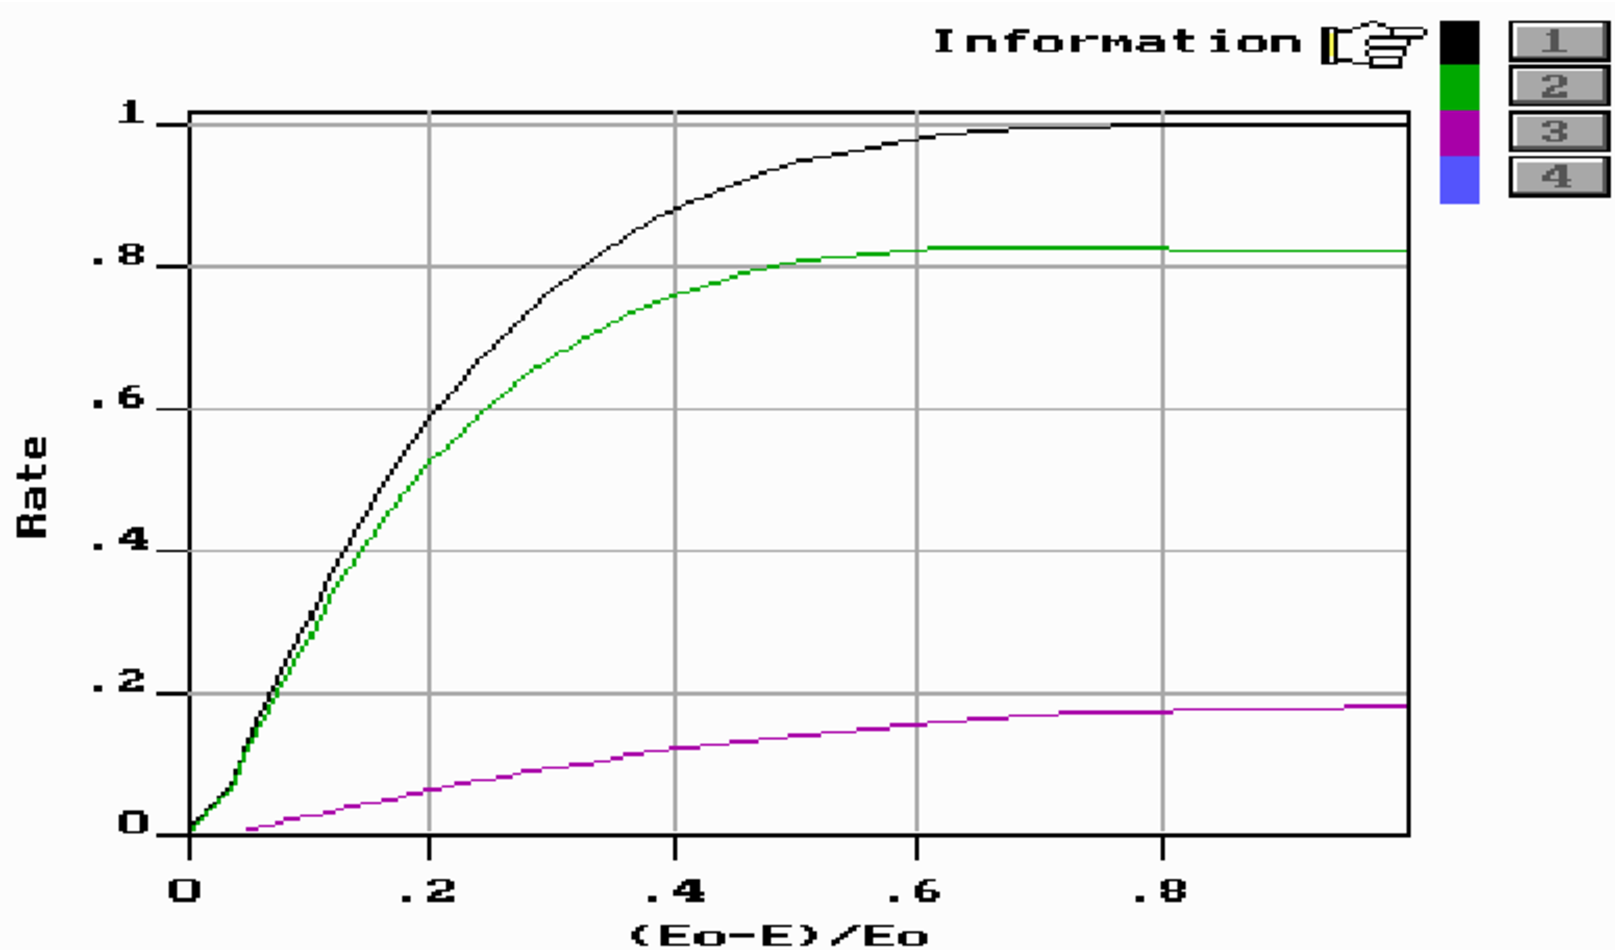
\includegraphics[width=.95\textwidth]{fluxes}
    \caption{Доля потоков электронов:
    1 -- электроны, перешедшие из налетающих в диффузионные;
2 -- дифундировавшие электроны с энергией $E$;
3 -- отраженные электроны с энергие от $E_0$ до $E$;
4 -- прошедшие насквозь через подложку электроны с энергией от $E_0$ до $E$.
}
    \label{fig:fluxes}
\end{figure}


По мере прохождения доля диффузионных электронов растёт.

\begin{figure}[h]
    \center
    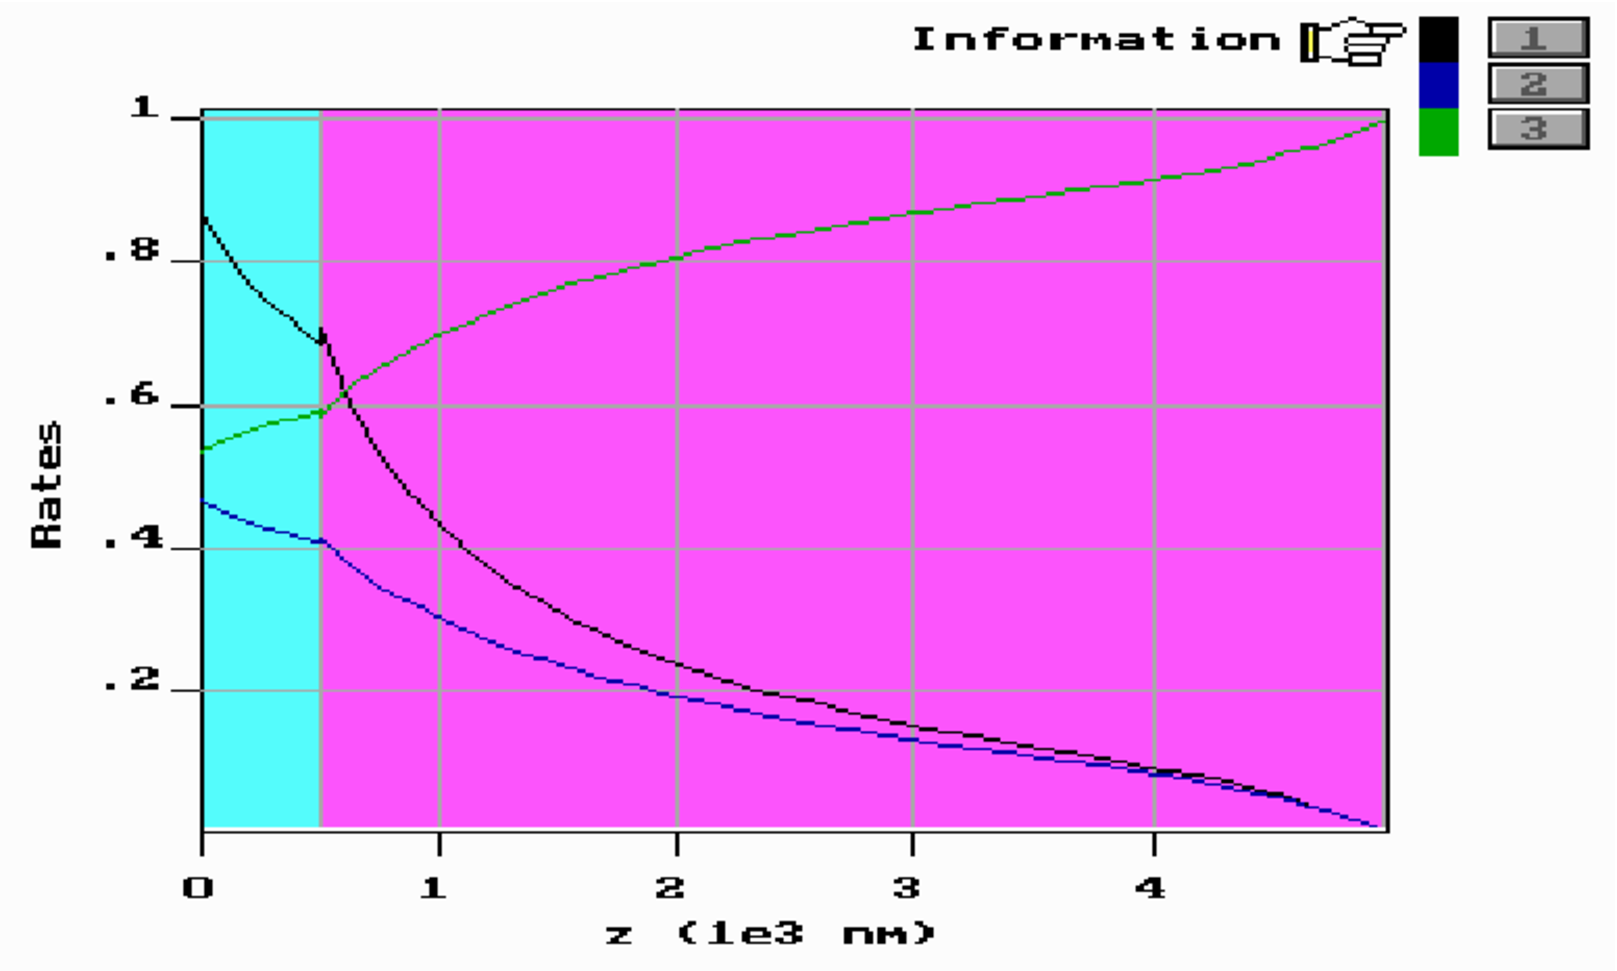
\includegraphics[width=.95\textwidth]{rates}
    \caption{Соотношение диффузионных и нерассеянных электронов: 1 -- отношение потока нерассеянных электронов к потоку диффузионных;
2 -- доля потока нерассеянных электронов;
3 -- доля потока диффузионных электронов.
}
    \label{fig:rates}
\end{figure}

При прохождении в глубь резиста, а впоследствии и подложки, пучок уширяется
\begin{figure}[h]
    \center
    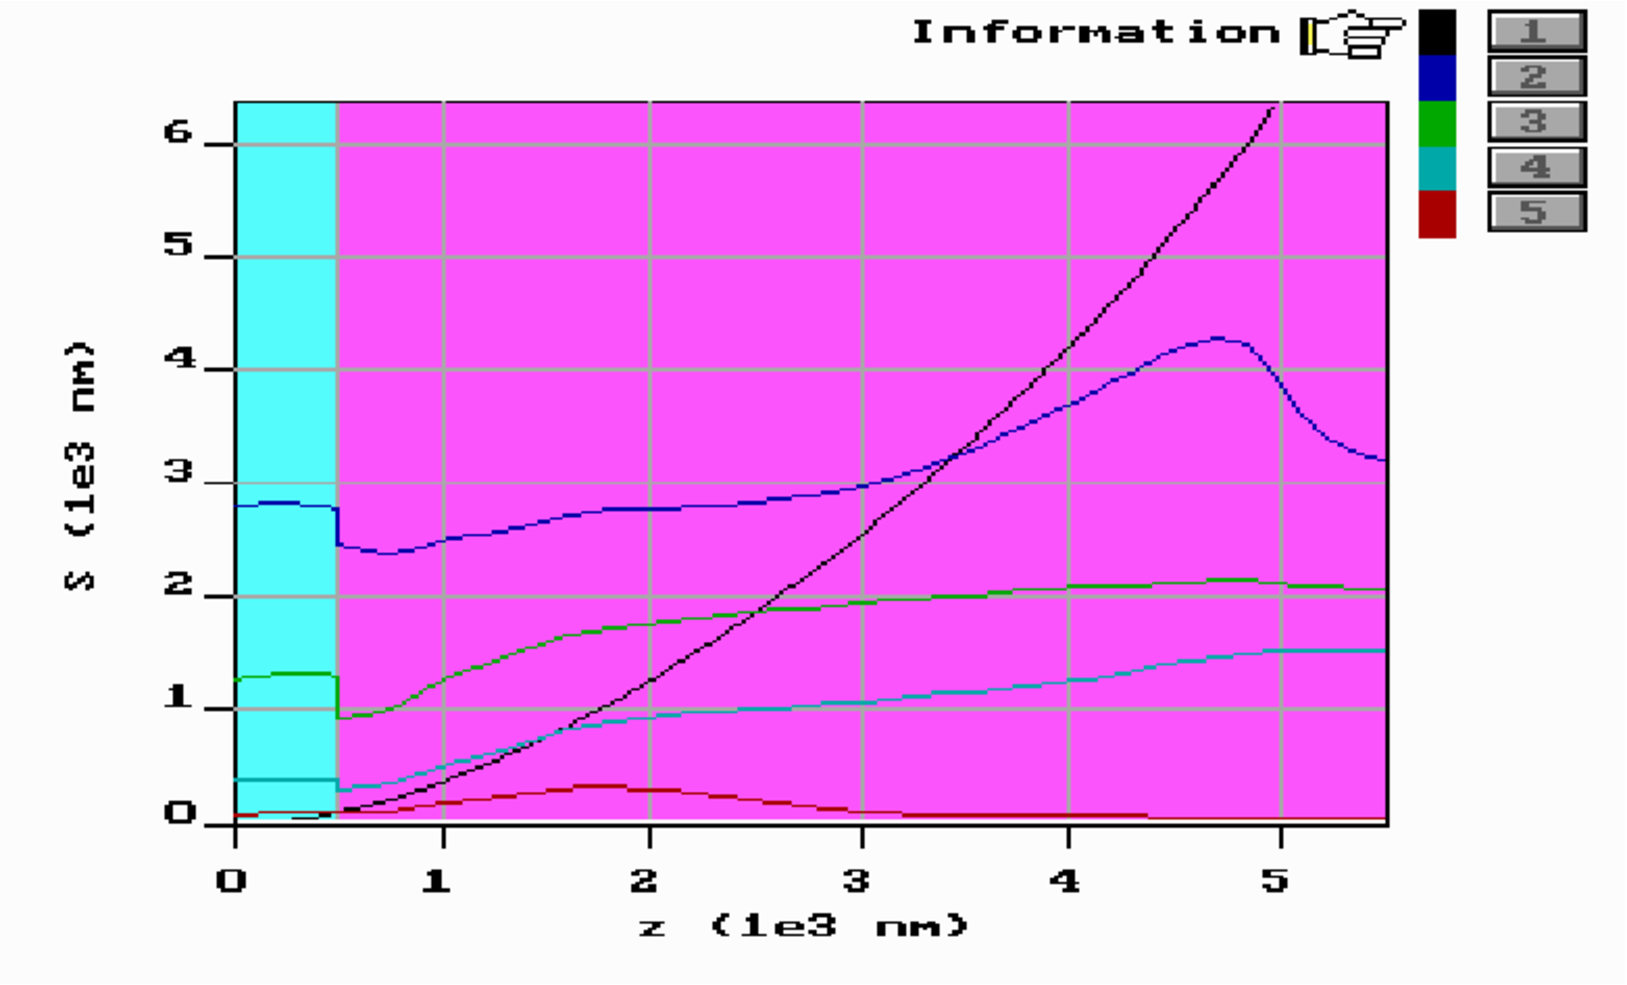
\includegraphics[width=.95\textwidth]{sequence}
    \caption{Поперечные размеры пучка:
1 -- полуширина пучка нерассеянных электронов;
2-5 -- полуширина пучка диффувзионных электронов по гауссиану}
    \label{fig:sequence}
\end{figure}


\begin{figure}[h]
    \center
    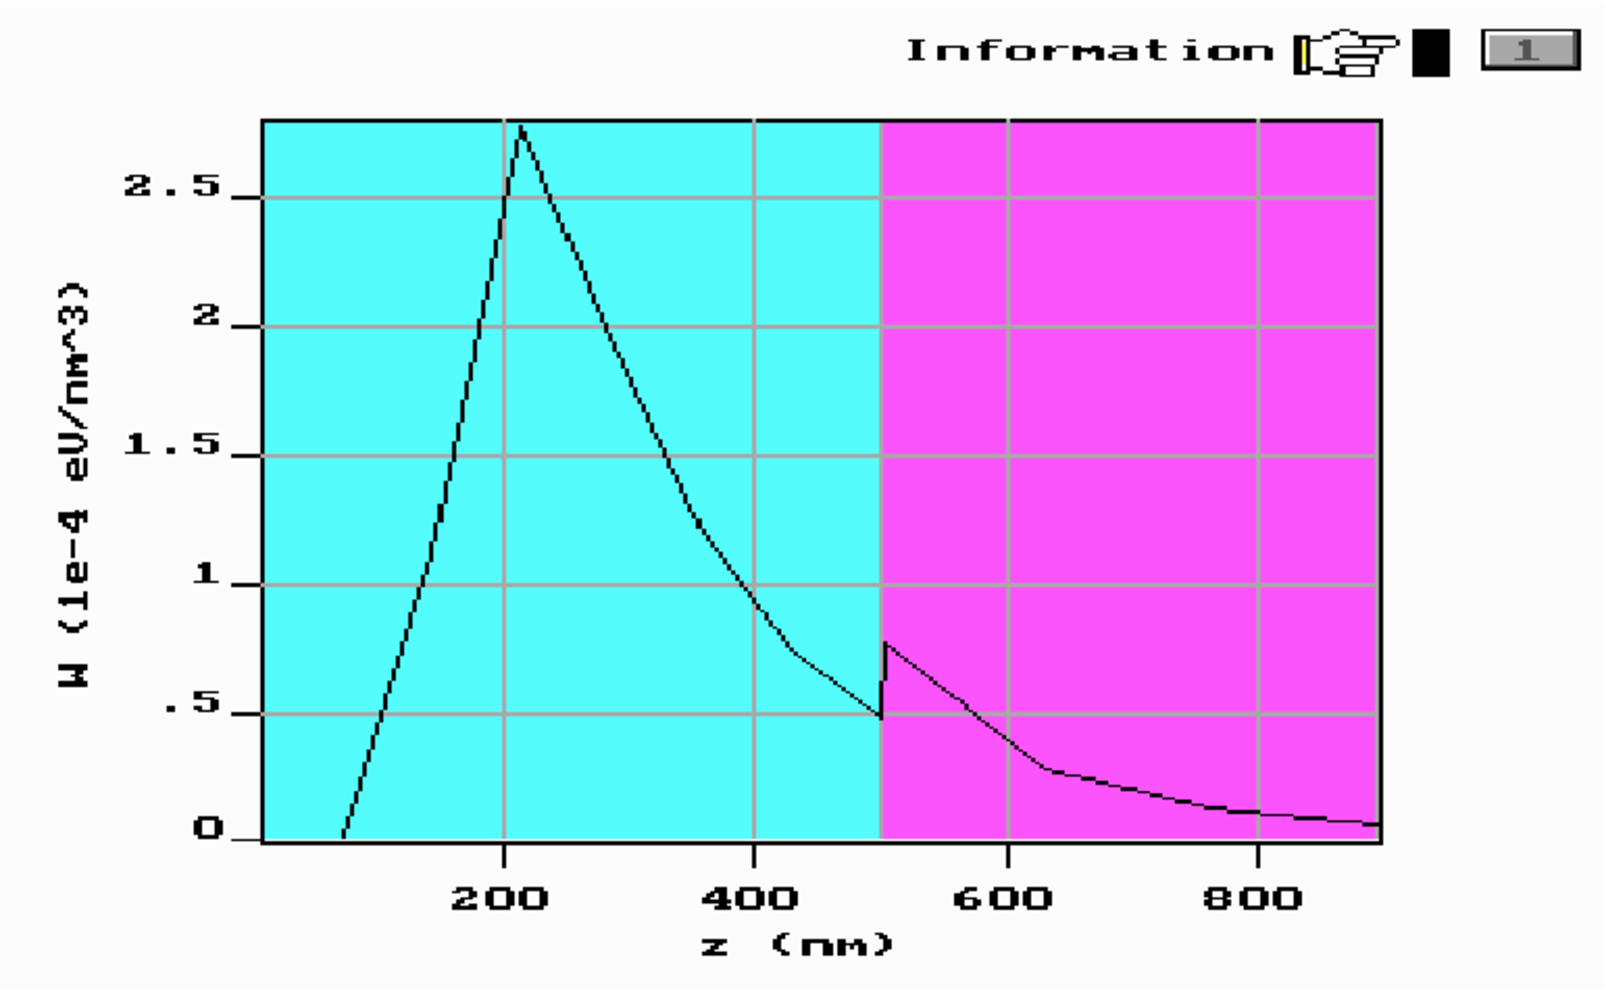
\includegraphics[width=.95\textwidth]{absorption}
    \caption{Зависимость от глубины плотности поглощенной энергии нерассеянных электрорнов в расчете на 1 электрон 1 для пучка радиусом 24.3 нм}
    \label{fig:absorption}
\end{figure}
